% CLAVE. Compiles with tectonic or a base TeX Live install:
%   tectonic paper.tex
\documentclass[11pt,a4paper]{article}

\usepackage[utf8]{inputenc}
\usepackage[T1]{fontenc}
\usepackage[margin=2.5cm]{geometry}
\usepackage{amsmath}
\usepackage{amssymb}
\usepackage{amsthm}
\usepackage{booktabs}
\usepackage{url}
\usepackage[hyphens]{xurl}
\usepackage{tikz}
\usepackage{pgfplots}
\usetikzlibrary{arrows.meta,decorations.pathreplacing,calligraphy,positioning,fit,backgrounds}
\pgfplotsset{compat=1.18}

\newtheorem{proposition}{Proposition}
\newtheorem{definition}{Definition}

\tikzset{
  actor/.style={draw, fill=black!5, rounded corners=2pt, minimum width=2.1cm,
                minimum height=0.6cm, align=center, inner sep=2pt},
  lifeline/.style={draw=black!45, dashed, line width=0.4pt},
  msg/.style={-{Latex[length=1.5mm,width=1.2mm]}, line width=0.6pt},
  mlab/.style={midway, above=1pt, align=center, font=\tiny, inner sep=1.5pt,
               fill=white},
  mlabb/.style={midway, below=1pt, align=center, font=\tiny, inner sep=1.5pt,
                fill=white},
  box/.style={draw, rounded corners=2pt, align=center, inner sep=4pt,
              font=\scriptsize},
  link/.style={draw, rounded corners=2pt, align=center, inner sep=3pt,
               font=\tiny, minimum height=0.75cm, text width=1.5cm},
}

\title{CLAVE: Custody-Less Accountable Verifiable Escrow}
\author{Rub\'en Sospedra}
\date{7 August 2026}

\begin{document}
\maketitle

\begin{abstract}
Platforms are increasingly required to identify their users, and they respond by
storing identity documents they then hold indefinitely. The resulting database is
a bulk surveillance capability wearing the costume of a targeted one. Refusing
access instead wins the technical argument and loses the legislative one.

We first establish why the obvious middle path fails. No platform that holds
sufficient key material can prove to a user that every use of that material was
published. The argument rules out an entire family of designs, including any
built on split keys, secure logs, or audited procedure, so long as one party
holds every share.

CLAVE takes the only remaining direction that recruits no partner: the platform
holds nothing. The user's device seals their legal identity against a public
threshold network the platform does not operate. The platform stores ciphertext.
A key for one account does not exist anywhere until a public on-chain request
causes the network to derive it, and that key opens exactly one account. The
network, not the platform, publishes a timelocked disclosure naming what was
opened, so silence cannot be extended by inaction.

We give the construction, state the relation proved at enrollment, and analyse
every link from the application binary through the circuit and the settlement
chain to the escrow keys, separating what rests on cryptographic hardness from
what rests on operational or economic assumptions. We contribute a verifiable
escrow proof with $41.51$ bits of soundness at the reference profile, eight
design decisions each stated with the failure it prevents, and a cost model.
Marginal cost is between \texttt{EUR} $1.6 \times 10^{-5}$ and
$8.2 \times 10^{-4}$ per registration, four to five orders of magnitude below
commercial identity verification.

A reference implementation accompanies this paper at
\url{https://clave.sospedra.me}. It runs the protocol end to end against a
mock settlement layer, and every figure below is emitted by one command. The
zero-knowledge circuit is the exception and is evaluated in the clear, which we
mark wherever it matters.
\end{abstract}

\section{Introduction}

Pseudonymity is being legislated away. Statutes now require identity checks
before ordinary online activity. Platforms comply by collecting passports, and
every breach corpus reads those collections for free.

The menu has two items. A surveillance database, or refusal. Refusal is correct
and it keeps losing, because the demand underneath is legitimate. Fraud drains
real accounts. Grooming happens in real conversations. Courts have real reasons
to ask who was behind an account.

This work assumes access will exist, by law or by contract, and asks a narrower
question. Given that the power exists, what must each use of it leave behind?

Certificate Transparency~\cite{rfc9162} made that move for certificates. Stop
preventing misissuance, start proving it happened. CONIKS~\cite{coniks} carried
it to key directories and named the honest guarantee as detection rather than
prevention. Transparency overlays~\cite{overlays} generalise the treatment. All
of them meet the same wall. A log proves what it contains. It cannot prove what
it omits.

Abelson \emph{et al.}~\cite{doormats} argued that mandated exceptional access
carries risks outweighing its benefits. We accept the technical analysis. The
political question did not settle, so the engineering question remains open.

We target three properties, stated so a non-specialist can hold a platform to
them:

\begin{enumerate}
  \item[P1] The identity bound to an account is sealed.
  \item[P2] It can be unsealed only if the unsealing is published.
  \item[P3] The published record carries a reference a human can check by hand.
\end{enumerate}

Section~\ref{sec:impossible} shows that no platform holding the key material can
offer P2, however carefully it is engineered. Sections~\ref{sec:construction}
onward give a construction in which the platform holds no key material at all,
and Section~\ref{sec:security} analyses what secures each link of it.

This paper contributes:

\begin{enumerate}
  \item an argument that custodial accountable pseudonymity is unachievable, and
        the three escape routes it leaves;
  \item CLAVE, a construction that takes one of them, with the platform holding
        only ciphertext;
  \item the enrollment relation stated formally, joining a credential proof to a
        verifiable escrow proof through one public commitment;
  \item a link-by-link security analysis from application binary to escrow key,
        separating cryptographic guarantees from operational ones; and
  \item a cost model showing marginal cost four to five orders of magnitude
        below commercial identity verification.
\end{enumerate}

\section{Why a custodian cannot do this}
\label{sec:impossible}

The natural design gives the platform a key, splits it in two, wraps every use in
an append-only log, and anchors the log publicly. That design cannot deliver P2,
and the reason is not an implementation flaw.

\begin{proposition}[Custodial impossibility]
No system in which a single party holds sufficient key material can guarantee to
a third party that every use of that material was published.
\end{proposition}

\begin{proof}[Argument]
Consider two worlds. In world A the platform follows the protocol and produces
public transcript $T$. In world B the platform produces the identical transcript
$T$, and also retains a copy of the plaintext, or a recovery key, or runs a
second instance of its own software. Any verifier observes exactly $T$ in both
worlds, so no function of $T$ separates them.
\end{proof}

Splitting the key across two modules the same party administers does not help,
because the party holds both shares. Logging every use does not help, because
the log records only what somebody chose to write. Anchoring the log does not
help, because anchoring fixes history rather than compelling entries.

Cryptography constrains what can be computed. It does not constrain whether a
computation happened in private. Publication is an act in the world, and forcing
it requires the decryption key to depend on a value that (i) the platform cannot
compute alone and (ii) comes into existence only when the record becomes public.

Exactly three sources satisfy both conditions. A threshold committee. Secure
hardware with remote attestation, where the trust root becomes a silicon vendor.
Witness encryption, which would satisfy the requirement exactly and does not
exist in deployable form.

\paragraph{Corollary.} The word "opening" needs care. Once plaintext reaches a
platform's storage it can be reread indefinitely with no cryptography involved.
The defensible event is the \emph{first} record-specific key release, never every
subsequent access. Any system claiming to log every access to an identity it
holds in the clear is claiming something it cannot enforce.

\section{Construction}
\label{sec:construction}

\subsection{Notation}

Let $\mathbb{G}_1, \mathbb{G}_2, \mathbb{G}_T$ be groups of prime order $r$ with
a bilinear pairing $e : \mathbb{G}_1 \times \mathbb{G}_2 \to \mathbb{G}_T$, and
let $P_1, P_2$ generate $\mathbb{G}_1, \mathbb{G}_2$. Write $[x]P$ for scalar
multiplication. Let $H_1 : \{0,1\}^* \to \mathbb{G}_1$ be a hash to the curve and
$H : \{0,1\}^* \to \{0,1\}^{256}$ a collision-resistant hash.

The escrow network holds a master secret $\mathsf{msk} \in \mathbb{Z}_r$ shared
among its nodes, and publishes $\mathsf{mpk} = [\mathsf{msk}]P_2$. For an
identity string $\mathsf{id}$ the corresponding key is

\begin{equation}
\mathsf{sk}_{\mathsf{id}} = [\mathsf{msk}]\,H_1(\mathsf{id}),
\label{eq:ibekey}
\end{equation}

which no party can compute without a threshold of shares. Encryption to
$\mathsf{id}$ follows Boneh and Franklin~\cite{bf}. Write
$\mathsf{Enc}_{\mathsf{id}}(m; \rho)$ for encryption with coins $\rho$ and
$\mathsf{Dec}_{\mathsf{sk}}(c)$ for decryption, which returns $\bot$ on failure.

\subsection{Parties and assumptions}

The adversary is the platform. It runs enrollment, storage, and its own
transparency record. It is rational and wants one account's identity without a
matching public entry.

\begin{enumerate}
  \item[A1] A threshold of the escrow network's nodes does not collude.
  \item[A2] The settlement chain does not reorganise below the finality depth set
        in policy.
  \item[A3] Bilinear Diffie-Hellman is hard in the chosen groups, discrete log is
        hard in $\mathbb{G}_1$, and $H$ is collision resistant.
  \item[A4] At least one party reads the published record against the chain, at
        least once. Continuous monitoring is not assumed.
  \item[A5] The passport chip's authentication key is not extractable.
  \item[A6] The user's device runs the software the platform published.
\end{enumerate}

A1, A2, A5 and A6 are not cryptographic. Section~\ref{sec:notcrypto} separates
them out explicitly, because a reader deserves to know which parts of the
construction rest on mathematics and which rest on people.

\subsection{Overview}

Figure~\ref{fig:arch} shows the four systems. The platform appears once and holds
no secret.

\begin{figure}[t]
\centering
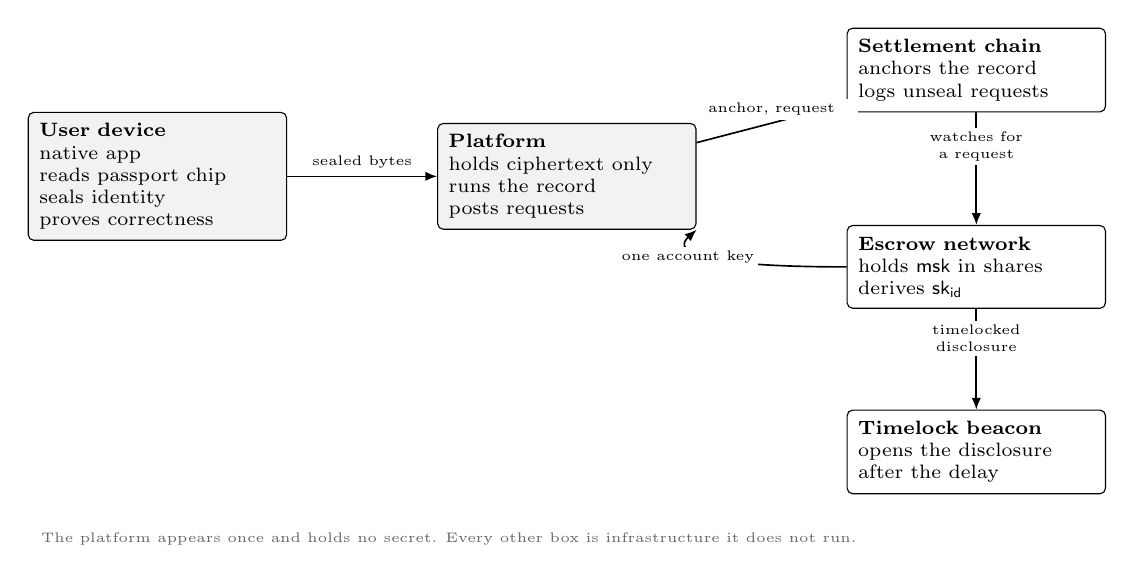
\begin{tikzpicture}[font=\scriptsize]

\node[box, fill=black!5, text width=3.0cm, align=left] (dev) at (0,0)
  {\textbf{User device}\\native app\\reads passport chip\\seals identity\\
   proves correctness};

\node[box, fill=black!5, text width=3.0cm, align=left] (op) at (5.2,0)
  {\textbf{Platform}\\holds ciphertext only\\runs the record\\posts requests};

\node[box, text width=3.0cm, align=left] (chain) at (10.4,1.35)
  {\textbf{Settlement chain}\\anchors the record\\logs unseal requests};

\node[box, text width=3.0cm, align=left] (net) at (10.4,-1.15)
  {\textbf{Escrow network}\\holds $\mathsf{msk}$ in shares\\derives
   $\mathsf{sk}_{\mathsf{id}}$};

\node[box, text width=3.0cm, align=left] (beacon) at (10.4,-3.5)
  {\textbf{Timelock beacon}\\opens the disclosure after the delay};

\draw[msg] (dev) -- node[mlab] {sealed bytes} (op);
\draw[msg] (op) -- node[mlab, text width=2.1cm] {anchor, request} (chain);
\draw[msg] (chain) -- node[mlab, text width=1.9cm] {watches for a request} (net);
\draw[msg] (net) -- node[mlab, text width=2.2cm] {timelocked disclosure} (beacon);
\draw[msg] (net.west) .. controls (6.6,-1.15) and (6.6,-0.9) ..
  node[mlabb, pos=0.75] {one account key} (op.south east);

\node[font=\tiny, text=black!60, anchor=west, align=left] at (-1.6,-4.6)
  {The platform appears once and holds no secret. Every other box is
   infrastructure it does not run.};

\end{tikzpicture}
\caption{The four systems. Only the chain is written to by the platform. The
escrow network is a set of machines that watches it. The beacon is a signing
service, not a chain. Deployable instances of all three exist today.}
\label{fig:arch}
\end{figure}

Figure~\ref{fig:lifecycle} follows the identity itself, from the passport to a
possible disclosure, and marks where each of the three properties holds. The
identity exists as plaintext in one place only, the user's device. Everywhere
else it is ciphertext or a public reference.

\begin{figure}[t]
\centering
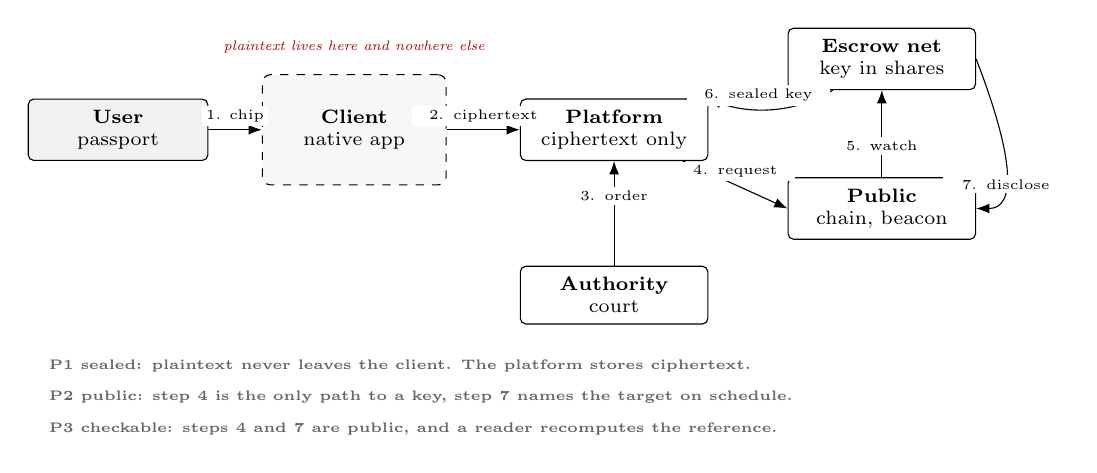
\begin{tikzpicture}[font=\scriptsize, >=Latex]

% actors
\node[box, fill=black!5, text width=2.0cm, align=center] (user) at (0,0)
  {\textbf{User}\\passport};
\node[draw, dashed, rounded corners=3pt, fill=black!3, text width=2.1cm,
      align=center, minimum height=1.4cm] (client) at (3.0,0)
  {\textbf{Client}\\native app};
\node[box, text width=2.1cm, align=center] (server) at (6.3,0)
  {\textbf{Platform}\\ciphertext only};
\node[box, text width=2.1cm, align=center] (network) at (9.7,0.9)
  {\textbf{Escrow net}\\key in shares};
\node[box, text width=2.1cm, align=center] (court) at (6.3,-2.1)
  {\textbf{Authority}\\court};
\node[box, text width=2.1cm, align=center] (public) at (9.7,-1.0)
  {\textbf{Public}\\chain, beacon};

\node[font=\tiny\itshape, text=red!70!black] at (3.0,1.05)
  {plaintext lives here and nowhere else};

\draw[->] (user) -- node[mlab] {1. chip} (client);
\draw[->] (client) -- node[mlab, text width=1.7cm] {2. ciphertext} (server);
\draw[->] (court) -- node[mlab, text width=1.6cm, pos=0.55] {3. order} (server);
\draw[->] (server) -- node[mlab, text width=1.4cm] {4. request} (public.west);
\draw[->] (public.north) -- node[mlabb] {5. watch} (network.south);
\draw[->] (network) .. controls (8.6,0.2) and (8.0,0.2) ..
  node[mlab, pos=0.6, text width=1.7cm] {6. sealed key} (server.north east);
\draw[->] (network.east) .. controls (11.4,-0.4) and (11.4,-1.0) ..
  node[mlabb, text width=1.5cm] {7. disclose} (public.east);

\node[font=\tiny\bfseries, text=black!60, anchor=west, align=left] at (-1.0,-3.0)
  {P1 sealed: plaintext never leaves the client. The platform stores ciphertext.};
\node[font=\tiny\bfseries, text=black!60, anchor=west, align=left] at (-1.0,-3.4)
  {P2 public: step 4 is the only path to a key, step 7 names the target on schedule.};
\node[font=\tiny\bfseries, text=black!60, anchor=west, align=left] at (-1.0,-3.8)
  {P3 checkable: steps 4 and 7 are public, and a reader recomputes the reference.};

\end{tikzpicture}
\caption{The lifecycle of one identity, and where the three properties hold.
The user's device is the only holder of plaintext. The platform holds
ciphertext. A key exists only after the platform posts a public request, step
4, and the escrow network, not the platform, publishes the disclosure at step
7. The authority is a third party that issues an order and holds no key.}
\label{fig:lifecycle}
\end{figure}

\subsection{Enrollment}

Enrollment runs entirely in a native application, because passport chips require
command exchanges that browser interfaces cannot issue. Figure~\ref{fig:enroll}
gives the order, and every arrow leaving the device carries ciphertext or a
proof.

\begin{figure}[t]
\centering
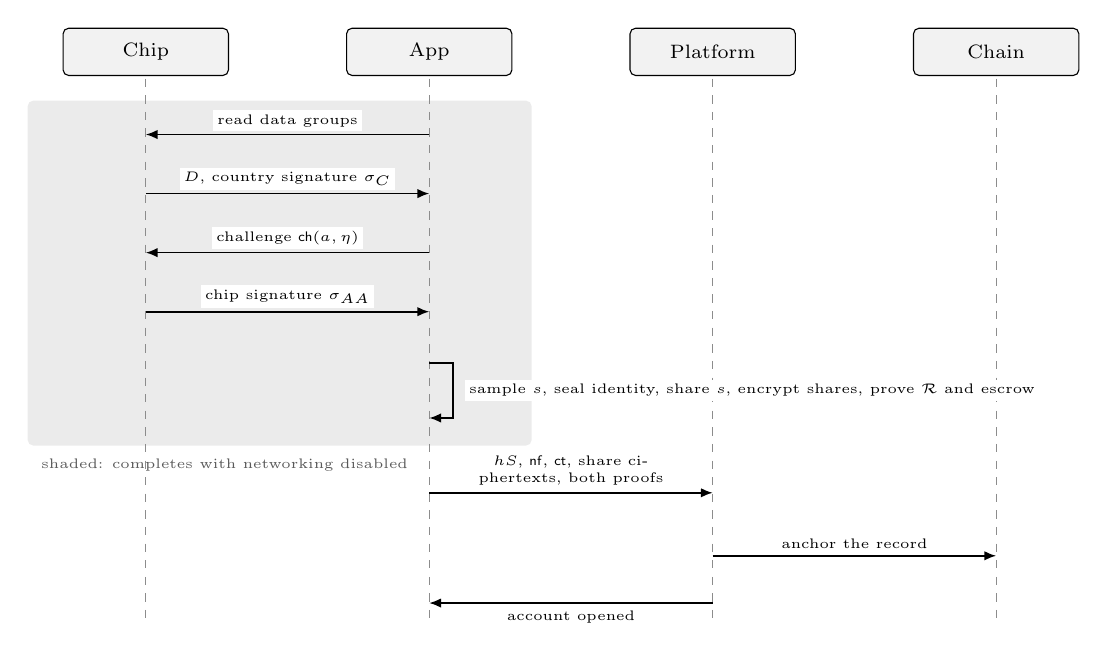
\begin{tikzpicture}[font=\scriptsize]

\foreach \i/\name in {0/{Chip}, 1/{App}, 2/{Platform}, 3/{Chain}} {
    \node[actor] (a\i) at (3.6*\i, 0) {\name};
    \draw[lifeline] (3.6*\i, -0.34) -- (3.6*\i, -7.2);
}

\begin{scope}[on background layer]
  \fill[black!8, rounded corners=2pt] (-1.5, -5.0) rectangle (4.9, -0.62);
\end{scope}
\node[font=\tiny, text=black!65, align=left, anchor=north west] at (-1.45, -5.05)
  {shaded: completes with networking disabled};

\draw[msg] (3.6, -1.05) -- node[mlab] {read data groups} (0, -1.05);
\draw[msg] (0, -1.8) -- node[mlab] {$D$, country signature $\sigma_C$} (3.6, -1.8);
\draw[msg] (3.6, -2.55) -- node[mlab] {challenge $\mathsf{ch}(a,\eta)$} (0, -2.55);
\draw[msg] (0, -3.3) -- node[mlab] {chip signature $\sigma_{AA}$} (3.6, -3.3);

\draw[msg] (3.6, -3.95) -- ++(0.3,0) -- ++(0,-0.7) -- ++(-0.3,0);
\node[font=\tiny, anchor=west, align=left, fill=white, inner sep=1.5pt]
  at (4.05, -4.3)
  {sample $s$, seal identity, share $s$, encrypt shares, prove $\mathcal{R}$
   and escrow};

\draw[msg] (3.6, -5.6) --
  node[mlab, text width=3.2cm] {$hS$, $\mathsf{nf}$, $\mathsf{ct}$, share
  ciphertexts, both proofs} (7.2, -5.6);
\draw[msg] (7.2, -6.4) -- node[mlab] {anchor the record} (10.8, -6.4);
\draw[msg] (7.2, -7.0) -- node[mlabb] {account opened} (3.6, -7.0);

\end{tikzpicture}
\caption{Enrollment. The identity never leaves the device. Sealing and proving
complete with no network, so a user may perform the whole shaded region in
airplane mode and reconnect only to transmit the result.}
\label{fig:enroll}
\end{figure}

The application reads the chip and requires Active Authentication or Chip
Authentication, so that a copied data dump does not suffice. The chip challenge
$\mathsf{ch}(a,\eta)$ derives from the account identifier $a$ and a single-use
server nonce $\eta$, and both are public inputs to the proof.

The application samples a uniform $s \in \mathbb{Z}_r$, seals the identity under
a key derived from $s$, shares $s$, encrypts each share to the escrow network,
and produces two proofs joined by the public value $hS = [s]P_1$.

\subsection{The enrollment relation}
\label{sec:relation}

\begin{definition}[Enrollment relation $\mathcal{R}$]
Public inputs are the account identifier $a$, the server nonce $\eta$, the
commitment $hS \in \mathbb{G}_1$, the nullifier $\mathsf{nf}$, the sealed
identity $\mathsf{ct}$, and the set $\mathcal{C}$ of trusted country signing
keys. The witness is the passport data $D$, the country signature $\sigma_C$,
the chip signature $\sigma_{AA}$, the scalar $s$, and the sealing nonce $\nu$.
$\mathcal{R}$ holds when all of the following hold.
\end{definition}

\begin{align}
&\exists\, \mathsf{pk}_C \in \mathcal{C} :
  \mathsf{Ver}(\mathsf{pk}_C,\, D,\, \sigma_C) = 1 \label{eq:r1}\\
&\mathsf{pk}_{AA} = \mathsf{extract}_{AA}(D) \label{eq:r2}\\
&\mathsf{Ver}(\mathsf{pk}_{AA},\, \mathsf{ch}(a,\eta),\, \sigma_{AA}) = 1
  \label{eq:r3}\\
&\mathsf{nf} = H(\mathsf{doc}(D) \,\|\, \mathsf{ctx}) \label{eq:r4}\\
&hS = [s]P_1 \label{eq:r5}\\
&\mathsf{ct} = \mathsf{AEAD.Enc}\big(\mathsf{kdf}(s),\, \nu,\,
  \mathsf{idb}(D),\, a\big) \label{eq:r6}
\end{align}

Each line does one job. Equation~\ref{eq:r1} establishes that a state issued the
document. Equation~\ref{eq:r2} takes the chip's authentication key from inside
the signed data, so that key inherits the country's signature.
Equation~\ref{eq:r3} establishes that the physical chip answered a challenge
bound to this account and this session, which a copied data dump cannot do.
Equation~\ref{eq:r4} derives the nullifier from the document alone, never from
$a$, so one document yields one account. Equations~\ref{eq:r5}
and~\ref{eq:r6} are the join: the identity signed by the state is exactly what is
sealed, under exactly the key committed by $hS$.

The last two carry the weight. Without \ref{eq:r6} a prover could present a
genuine passport and seal unrelated bytes, and both proofs would verify
independently. Because $D$ feeds \ref{eq:r1} and \ref{eq:r6} through the same
witness wires, no such separation exists.

\subsection{The verifiable escrow proof}
\label{sec:escrowproof}

$\mathcal{R}$ says the identity is sealed under $s$. It says nothing about
whether $s$ can ever be recovered. That is the escrow proof's job.

Proving pairing-based encryption correct inside a general proof system is
expensive, so we use cut-and-choose. The prover shares $s$ into $n$ shares at
threshold $k$~\cite{shamir} using a polynomial $f$ of degree $k-1$ with
$f(0) = s$, publishes Feldman commitments $C_j = [c_j]P_1$ to the coefficients of
$f$~\cite{feldman}, and encrypts each share to the account's identity string:

\begin{equation}
E_i = \mathsf{Enc}_{\mathsf{id}_a}(f(i);\, \rho_i), \qquad i = 1,\dots,n.
\end{equation}

A challenge is derived by Fiat-Shamir~\cite{fiatshamir} over the entire
statement, before any opening:

\begin{equation}
\mathcal{O} = \mathsf{select}_o\Big(
  H\big(\, a \,\|\, hS \,\|\, C_0 \cdots C_{k-1} \,\|\, E_1 \cdots E_n \,\|\,
  \mathsf{params} \,\big)\Big).
\label{eq:challenge}
\end{equation}

For each $i \in \mathcal{O}$ the prover reveals $f(i)$ and $\rho_i$, and the
verifier performs two checks:

\begin{align}
[f(i)]P_1 &\overset{?}{=} \textstyle\sum_{j=0}^{k-1} [\,i^{\,j}\,] C_j
  \label{eq:feldman}\\
E_i &\overset{?}{=} \mathsf{Enc}_{\mathsf{id}_a}(f(i);\, \rho_i)
  \label{eq:recompute}
\end{align}

Equation~\ref{eq:feldman} binds the share to the polynomial.
Equation~\ref{eq:recompute} binds the polynomial to the published bytes. Omitting
the second is the most likely implementation error, because the first looks
sufficient and is not. The verifier also checks $C_0 = hS$, which is the join
back to $\mathcal{R}$. Figure~\ref{fig:escrow} shows one round.

\begin{figure}[t]
\centering
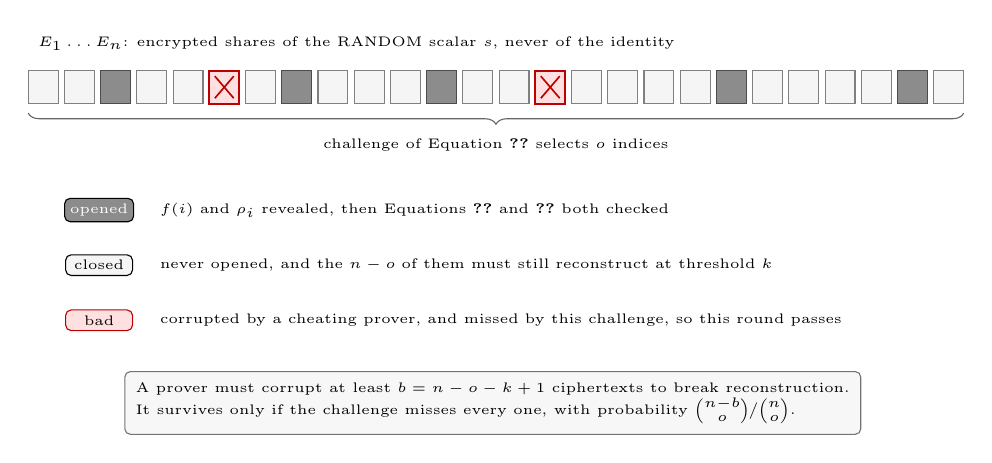
\begin{tikzpicture}[font=\scriptsize]

\def\cw{0.46}
\foreach \i in {0,...,25} {
  \draw[fill=black!4, draw=black!50, line width=0.4pt]
    (\cw*\i, 0) rectangle (\cw*\i+0.38, 0.42);
}
\foreach \i in {2,7,11,19,24} {
  \draw[fill=black!45, draw=black!70, line width=0.4pt]
    (\cw*\i, 0) rectangle (\cw*\i+0.38, 0.42);
}
\foreach \i in {5,14} {
  \draw[fill=red!12, draw=red!75!black, line width=0.8pt]
    (\cw*\i, 0) rectangle (\cw*\i+0.38, 0.42);
  \draw[red!75!black, line width=0.6pt]
    (\cw*\i+0.07, 0.07) -- (\cw*\i+0.31, 0.35);
  \draw[red!75!black, line width=0.6pt]
    (\cw*\i+0.07, 0.35) -- (\cw*\i+0.31, 0.07);
}

\node[font=\tiny, anchor=south west] at (0, 0.55)
  {$E_1 \dots E_n$: encrypted shares of the RANDOM scalar $s$, never of the
   identity};

\draw[decorate, decoration={brace, amplitude=4pt, mirror}, black!60]
  (0, -0.12) -- (11.88, -0.12);
\node[font=\tiny, anchor=north] at (5.94, -0.32)
  {challenge of Equation~\ref{eq:challenge} selects $o$ indices};

\node[box, fill=black!45, text=white, minimum width=0.85cm, inner sep=2pt,
      font=\tiny] at (0.9, -1.35) {opened};
\node[font=\tiny, anchor=west, align=left, text width=9.6cm] at (1.55, -1.35)
  {$f(i)$ and $\rho_i$ revealed, then Equations~\ref{eq:feldman}
   and~\ref{eq:recompute} both checked};

\node[box, fill=black!4, minimum width=0.85cm, inner sep=2pt, font=\tiny]
  at (0.9, -2.05) {closed};
\node[font=\tiny, anchor=west, align=left, text width=9.6cm] at (1.55, -2.05)
  {never opened, and the $n-o$ of them must still reconstruct at threshold $k$};

\node[box, fill=red!12, draw=red!75!black, minimum width=0.85cm, inner sep=2pt,
      font=\tiny] at (0.9, -2.75) {bad};
\node[font=\tiny, anchor=west, align=left, text width=9.6cm] at (1.55, -2.75)
  {corrupted by a cheating prover, and missed by this challenge, so this round
   passes};

\node[box, draw=black!55, fill=black!3, align=left, font=\tiny]
  at (5.9, -3.8)
  {A prover must corrupt at least $b = n - o - k + 1$ ciphertexts to break
   reconstruction.\\
   It survives only if the challenge misses every one, with probability
   $\binom{n-b}{o} \big/ \binom{n}{o}$.};

\end{tikzpicture}
\caption{One round of the cut-and-choose, drawn with 26 cells for legibility.
The reference profile uses $n = 130$, $k = 27$ and $o = 26$. Opening $o = 26$
reveals fewer shares than the threshold $k = 27$, so the openings leak nothing
about $s$.}
\label{fig:escrow}
\end{figure}

\subsection{Custody}

The escrow master secret is held by a public threshold network that the platform
does not operate and does not pay per transaction. Several such networks run
today, offering release conditioned on observable on-chain events. The platform
holds no share of $\mathsf{msk}$.

A deployment may spread shares across several independent networks and require
all of them, which raises the bar for collusion at the cost of survivability if
one ceases operation. Section~\ref{sec:limits} argues this is the most
consequential deployment parameter.

\subsection{Unsealing and disclosure}

Figure~\ref{fig:unseal} gives the sequence and its timing.

\begin{figure}[t]
\centering
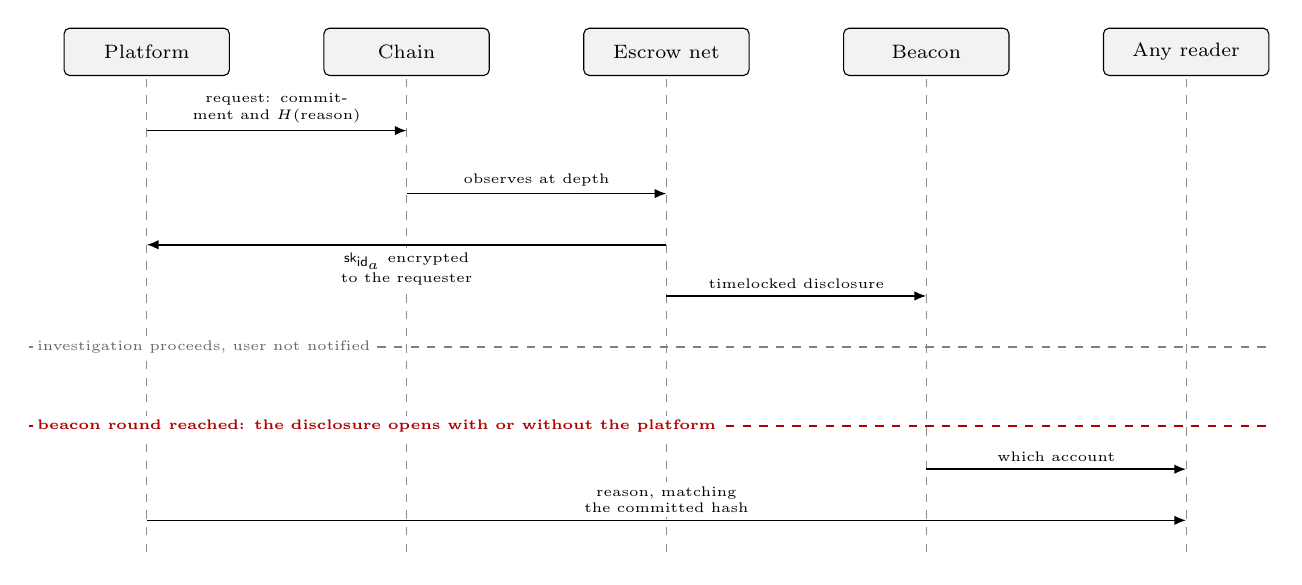
\begin{tikzpicture}[font=\scriptsize]

\foreach \i/\name in {0/{Platform}, 1/{Chain}, 2/{Escrow net}, 3/{Beacon},
                      4/{Any reader}} {
    \node[actor] (a\i) at (3.3*\i, 0) {\name};
    \draw[lifeline] (3.3*\i, -0.34) -- (3.3*\i, -6.4);
}

\draw[msg] (0, -1.0) --
  node[mlab, text width=2.7cm] {request: commitment and $H(\text{reason})$}
  (3.3, -1.0);
\draw[msg] (3.3, -1.8) -- node[mlab] {observes at depth} (6.6, -1.8);
\draw[msg] (6.6, -2.45) --
  node[mlabb, text width=3.0cm] {$\mathsf{sk}_{\mathsf{id}_a}$ encrypted to the
  requester} (0, -2.45);
\draw[msg] (6.6, -3.1) --
  node[mlab, text width=2.5cm] {timelocked disclosure} (9.9, -3.1);

\draw[dashed, black!50, line width=0.6pt] (-1.5, -3.75) -- (14.3, -3.75);
\node[font=\tiny, anchor=west, fill=white, inner sep=1.5pt, text=black!60]
  at (-1.45, -3.75) {investigation proceeds, user not notified};

\draw[dashed, red!70!black, line width=0.7pt] (-1.5, -4.75) -- (14.3, -4.75);
\node[font=\tiny\bfseries, anchor=west, fill=white, inner sep=1.5pt,
      text=red!70!black] at (-1.45, -4.75)
  {beacon round reached: the disclosure opens with or without the platform};

\draw[msg] (9.9, -5.3) -- node[mlab] {which account} (13.2, -5.3);
\draw[msg] (0, -5.95) --
  node[mlab, text width=2.9cm] {reason, matching the committed hash} (13.2, -5.95);

\end{tikzpicture}
\caption{Unsealing. The count of requests is public from the first message. The
target becomes public when the beacon reaches the sealed round, whether or not
the platform cooperates. The reason was fixed by its hash at request time, so it
cannot be revised once the outcome is known.}
\label{fig:unseal}
\end{figure}

The escrow network encrypts $\mathsf{sk}_{\mathsf{id}_a}$ to the requester key
committed in the same transaction, never publishing it in the clear, because a
published key would expose the user's identity to everyone rather than to the
authority that asked.

Recovery is not simply decrypt and reconstruct. Given
$\mathsf{sk}_{\mathsf{id}_a}$, a recovering party computes
$\sigma_i = \mathsf{Dec}_{\mathsf{sk}}(E_i)$ for successive $i \notin
\mathcal{O}$, discards any $\sigma_i = \bot$, retains only those satisfying
Equation~\ref{eq:feldman}, and stops once it holds $k$ of them, indexed by a set
$S$. It then interpolates

\begin{equation}
s' = \sum_{i \in S} \sigma_i \prod_{j \in S \setminus \{i\}}
  \frac{j}{\,j - i\,} \pmod r,
\label{eq:lagrange}
\end{equation}

and accepts only if $[s']P_1 = hS$. Taking the first $k$ decryptions without
checking each against Equation~\ref{eq:feldman} is unsafe, because cut-and-choose
does not promise that every unopened ciphertext is well formed. At most
$n - o + 1$ decryptions are needed.

\subsection{Client integrity}
\label{sec:client}

The application holds the plaintext while it works, so no cryptography prevents
it from transmitting it. What the design provides is detectability. Platform
attestation gates enrollment, so a repackaged application cannot enroll, which
defends against third-party tampering and provides nothing against a hostile
first party.

Three checks are available to a user without expertise. Observe the
application's network traffic, which is why certificates are not pinned. Enroll
with networking disabled, since sealing requires none. Rebuild from published
source where the platform permits it.

\section{Security analysis}
\label{sec:security}

\subsection{Soundness of the escrow proof}

A cheating prover corrupts some set of $b$ ciphertexts, hoping the challenge
misses all of them. Reconstruction from the unopened set requires $k$ good shares
out of $n-o$, so breaking recovery requires

\begin{equation}
b \ \geq\ n - o - k + 1.
\label{eq:bmin}
\end{equation}

Such a prover passes only when $\mathcal{O}$ avoids every corrupted index, which
happens with probability

\begin{equation}
\Pr[\text{pass}] \ =\ \binom{n-b}{o} \Big/ \binom{n}{o},
\label{eq:ppass}
\end{equation}

giving soundness in bits

\begin{equation}
\lambda \ =\ \log_2 \binom{n}{o} \ -\ \log_2 \binom{n-b}{o}.
\label{eq:soundness}
\end{equation}

At the reference profile $n = 130$, $k = 27$, $o = 26$, Equation~\ref{eq:bmin}
gives $b = 78$ and Equation~\ref{eq:soundness} gives $\lambda = 41.51$ bits.

Figure~\ref{fig:cheating} plots Equation~\ref{eq:ppass} against $b$ and shows why
the scheme is not weak at small $b$ in any way that matters. Corrupting a single
ciphertext succeeds with probability $0.80$, and achieves nothing, because 129
good ciphertexts remain and recovery still succeeds. Only at $b = 78$ does
success mean the secret is unrecoverable, and there the probability is
$3.19 \times 10^{-13}$.

\begin{figure}[t]
\centering
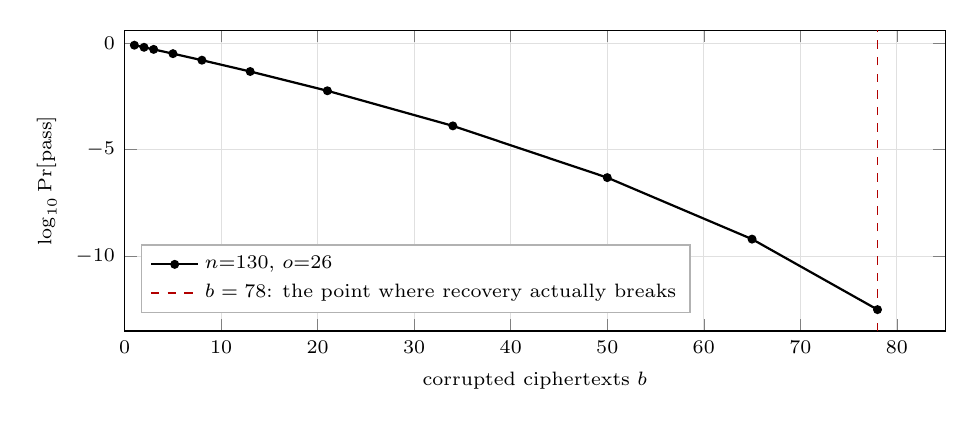
\begin{tikzpicture}
\begin{axis}[
  width=12cm, height=5.4cm,
  xlabel={corrupted ciphertexts $b$},
  ylabel={$\log_{10} \Pr[\text{pass}]$},
  xmin=0, xmax=85, ymin=-13.5, ymax=0.6,
  grid=major, grid style={black!12},
  tick label style={font=\scriptsize},
  label style={font=\scriptsize},
  legend style={font=\scriptsize, at={(0.02,0.06)}, anchor=south west,
                draw=black!30},
  legend cell align=left,
]
\addplot[black, line width=0.8pt, mark=*, mark size=1.2pt] coordinates {
  (1,-0.097) (2,-0.195) (3,-0.293) (5,-0.493) (8,-0.800) (13,-1.330)
  (21,-2.234) (34,-3.880) (50,-6.306) (65,-9.191) (78,-12.497)
};
\addlegendentry{$n{=}130$, $o{=}26$}
\addplot[dashed, red!70!black, line width=0.7pt, mark=none] coordinates {
  (78,-13.5) (78,0.6)
};
\addlegendentry{$b = 78$: the point where recovery actually breaks}
\end{axis}
\end{tikzpicture}
\caption{Probability that a cheating prover survives one round, against how many
ciphertexts it corrupted. Low $b$ passes easily and accomplishes nothing.
Recovery only fails from $b = 78$, where the probability is
$3.19 \times 10^{-13}$.}
\label{fig:cheating}
\end{figure}

Equation~\ref{eq:soundness} gives pre-query soundness. A prover may discard a
transcript and retry with fresh randomness until it draws a favourable challenge,
so a deployment must include grinding in its budget: with $q$ attempts the bound
degrades to roughly $q \cdot 2^{-\lambda}$. At the reference profile each attempt
requires recomputing $n$ pairing-based encryptions, which makes a useful $q$
economically infeasible, but the figure must be labelled for what it is.

Table~\ref{tab:soundness} and Figure~\ref{fig:soundness} give the parameter
space.

\subsection{Measured cost of the escrow proof}

Table~\ref{tab:measured} reports the reference implementation at the reference
profile. These are measurements rather than estimates, and unlike the soundness
figures they are host specific.

\begin{table}[h]
\centering
\begin{tabular}{lr}
\toprule
Operation, $n{=}130$, $k{=}27$, $o{=}26$ & Cost \\
\midrule
Prove, on the user's device            & $\approx$ 1800 ms \\
Verify, on the platform                & $\approx$ 2400 ms \\
Recover, given the derived key         & $\approx$ 2400 ms \\
Decryptions used during recovery       & 27 of at most 105 \\
Enrollment record size                 & $\approx$ 30{,}500 bytes \\
\midrule
Seal on device, whole enrollment       & $\approx$ 1700 ms \\
Platform accept, both proofs           & $\approx$ 2400 ms \\
\bottomrule
\end{tabular}
\caption{Measured on an Apple M5 Pro, Node v24.18.0. Recovery needed 27
decryptions against a worst case of 105, because it stops as soon as it holds
$k$ shares that pass Equation~\ref{eq:feldman}. The record is an order of
magnitude smaller than the 50 KB the cost model of Section 8 assumes, so that
model is conservative.}
\label{tab:measured}
\end{table}

Two observations. Recovery cost is dominated by pairing operations and scales
with $k$ rather than $n$, which is why it used 27 decryptions and not 105. And
the measured record size of about 30 KB is well under the 50 KB the cost model
assumes, so the per-registration figures in Section 8 overstate storage by
roughly forty percent.

\begin{table}[h]
\centering
\begin{tabular}{lrrr}
\toprule
Profile & $b$ & Soundness (bits) & Worst-case decryptions \\
\midrule
$n{=}24$, $k{=}7$, $o{=}6$    & 12 &  7.19 &  19 \\
$n{=}120$, $k{=}25$, $o{=}24$ & 72 & 38.29 &  97 \\
$n{=}126$, $k{=}26$, $o{=}25$ & 76 & 40.22 & 102 \\
$n{=}130$, $k{=}27$, $o{=}26$ & 78 & 41.51 & 105 \\
\bottomrule
\end{tabular}
\caption{Escrow proof parameters, from Equations~\ref{eq:bmin}
and~\ref{eq:soundness}. The last row is the reference profile.}
\label{tab:soundness}
\end{table}

\begin{figure}[t]
\centering
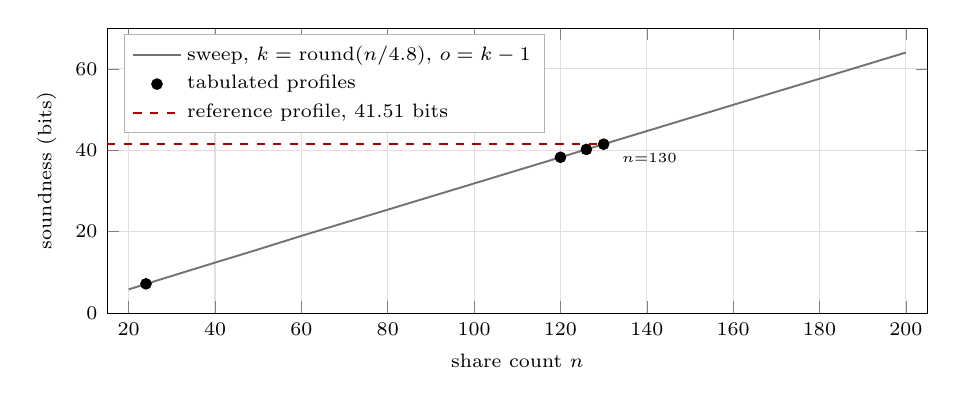
\begin{tikzpicture}
\begin{axis}[
  width=12cm, height=5.2cm,
  xlabel={share count $n$},
  ylabel={soundness (bits)},
  xmin=15, xmax=205, ymin=0, ymax=70,
  grid=major, grid style={black!12},
  tick label style={font=\scriptsize},
  label style={font=\scriptsize},
  legend style={font=\scriptsize, at={(0.02,0.98)}, anchor=north west,
                draw=black!30},
  legend cell align=left,
]
\addplot[black!55, line width=0.7pt, mark=none] coordinates {
  (20,5.83) (30,9.14) (40,12.41) (50,15.65) (60,18.98) (70,22.20)
  (80,25.42) (90,28.64) (100,31.86) (110,35.08) (120,38.29) (130,41.51)
  (140,44.73) (150,47.95) (160,51.17) (170,54.39) (180,57.59) (190,60.81)
  (200,64.03)
};
\addlegendentry{sweep, $k = \mathrm{round}(n/4.8)$, $o = k-1$}
\addplot[only marks, mark=*, mark size=1.9pt, black] coordinates {
  (24,7.19) (120,38.29) (126,40.22) (130,41.51)
};
\addlegendentry{tabulated profiles}
\addplot[dashed, red!70!black, line width=0.6pt, mark=none] coordinates {
  (15,41.51) (130,41.51)
};
\addlegendentry{reference profile, 41.51 bits}
\node[font=\tiny, anchor=north west] at (axis cs:132,41.51) {$n{=}130$};
\end{axis}
\end{tikzpicture}
\caption{Soundness against share count, from Equation~\ref{eq:soundness}. Linear
in $n$ once the opened fraction is fixed. One more bit costs about 3.1 more
shares and about 2.5 more decryptions at recovery.}
\label{fig:soundness}
\end{figure}

\subsection{The evidence standard}
\label{sec:evidence}

The reference implementation carries 49 tests and a mutation gate over 22
guards. The gate breaks each guard in turn, reruns the tests, and fails if the
suite stays green. At submission every test passes and no mutation survives. A
passing suite shows the checks accept honest input. A surviving mutation would
show a check that no test defends, and there are none.

Table~\ref{tab:claims} maps each property this paper asserts to the artifact
that establishes it. Four kinds appear. A \emph{formula} is computed and
reproduces on every host. A \emph{test} is a runnable assertion. A
\emph{mutation} names a guard whose deletion reddens a named test. A
\emph{gap} is a property the implementation does not establish, carried in
Section~\ref{sec:limits} and never dressed as proven.

\begin{table}[h]
\centering
\scriptsize
\setlength{\tabcolsep}{4pt}
\begin{tabular}{p{5.0cm}p{1.6cm}p{5.0cm}}
\toprule
Property & Evidence & Artifact \\
\midrule
Soundness $\lambda = 41.51$ bits at $n{=}130$ & formula &
  Eq.~\ref{eq:soundness}, reproduced exactly \\
Corruption floor $b = n-o-k+1$ & formula, test &
  Eq.~\ref{eq:bmin}, ``Equation 2'' \\
Low corruption passes and gains nothing & formula, test &
  Fig.~\ref{fig:cheating}, ``Figure 5'' \\
Opened share lies on the polynomial & mutation &
  \texttt{escrow:feldman-check} \\
Published bytes recompute from coins & mutation &
  \texttt{escrow:ciphertext-\allowbreak recomputation} \\
Recovery validates each candidate, fails closed & mutation &
  \texttt{escrow:recovery-\allowbreak validates-\allowbreak candidates} \\
Openings leak nothing, $o < k$ enforced & mutation &
  \texttt{escrow:openings-below-threshold} \\
Escrow proof binds to the credential commitment & mutation &
  \texttt{escrow:c0-equals-hs} \\
Sealed identity opens only from the secret, not its
public commitment & mutation &
  \texttt{relation:seal-key-from-secret} \\
Sealed bytes are the state-signed identity & mutation &
  \texttt{relation:seal-binding} \\
Only a trusted country signature is accepted & mutation &
  \texttt{relation:country-signature} \\
Chip response is bound to one account & mutation &
  \texttt{relation:chip-presence} \\
Hash preimages are length-framed & mutation &
  \texttt{relation:challenge-framed} \\
One document enrolls once & mutation &
  \texttt{protocol:nullifier-uniqueness} \\
Credential proof is account-bound & mutation &
  \texttt{protocol:credential-\allowbreak account-binding} \\
No key without a confirmed on-chain request & mutation, test &
  \texttt{protocol:request-must-be-confirmed} \\
Keys derivable equal requests, one to one & test &
  ``claim 2: one to one'' \\
Reason is bound to its on-chain hash & mutation &
  \texttt{protocol:reason-matches-commitment} \\
Disclosure schedule is network policy & mutation &
  \texttt{protocol:policy-owns-\allowbreak disclosure-round} \\
A key opens exactly one account & test &
  ``Proposition 3'' \\
Platform stores no plaintext & test &
  ``stores no plaintext'', ``no wrong key recovers'' \\
Reference recomputes from public data & test &
  ``claim 3: recomputes from public data'' \\
Beacon refuses an out-of-range round & mutation &
  \texttt{beacon:round-validated} \\
\midrule
Zero-knowledge of the credential proof & gap &
  circuit absent, Sec.~\ref{sec:limits} \\
Non-collusion of the escrow network & gap &
  single process, Sec.~\ref{sec:limits} \\
Client runs the published code & gap &
  detectable not preventable, Sec.~\ref{sec:limits} \\
Physical chip present, not a dump & gap &
  passive authentication, Sec.~\ref{sec:limits} \\
\bottomrule
\end{tabular}
\caption{Every asserted property against the artifact that establishes it. The
four gaps are stated, never proven, and none is dressed as a result.}
\label{tab:claims}
\end{table}

\subsection{Confidentiality before release}

\begin{proposition}[The openings leak nothing]
The $o$ revealed shares are values of a degree $k{-}1$ polynomial at $o < k$
distinct points. For any candidate $s^{*} \in \mathbb{Z}_r$ there is exactly one
polynomial of degree $k{-}1$ agreeing with those shares and having
$f(0) = s^{*}$. The openings are therefore independent of $s$.
\end{proposition}

The Feldman commitments do reveal $C_0 = [s]P_1$, so $s$ is only as hidden as
discrete log in $\mathbb{G}_1$. This is exactly why $s$ must be a uniform scalar
and not the identity. A commitment to a low-entropy value is a target for offline
enumeration, and identity data is low entropy: document numbers are short, and
names and birth dates already appear in breach corpora. Sealing the identity
under $\mathsf{kdf}(s)$ and committing only to $s$ removes that attack.

\begin{proposition}[Platform confidentiality]
Under A1 and A3, a platform holding $\{E_i\}$, $\{C_j\}$, $hS$ and $\mathsf{ct}$
learns nothing about the identity beyond the length of $\mathsf{ct}$.
\end{proposition}

Recovering the identity requires $\mathsf{kdf}(s)$, hence $s$, hence $k$ shares,
hence $\mathsf{sk}_{\mathsf{id}_a}$, hence a threshold of $\mathsf{msk}$ shares
under Equation~\ref{eq:ibekey}. Deriving $\mathsf{sk}_{\mathsf{id}_a}$ from
$\mathsf{mpk}$ alone is the bilinear Diffie-Hellman problem.

\subsection{Per-account scoping}

\begin{proposition}[A key opens one account]
$\mathsf{sk}_{\mathsf{id}_a}$ decrypts ciphertexts under $\mathsf{id}_a$ and no
others. Using it against $\mathsf{id}_{a'}$ for $a' \neq a$ requires
$[\mathsf{msk}]H_1(\mathsf{id}_{a'})$, which by Equation~\ref{eq:ibekey} is a
different group element with no efficient relation to the first.
\end{proposition}

This is the property P2 depends on. Opening $N$ accounts requires $N$ derivations,
each triggered by its own public request. Bulk access produces bulk public
evidence, and no key exists whose possession opens more than one person.

\subsection{The chain of custody, link by link}

Figure~\ref{fig:trustchain} follows one enrollment from the application binary to
a released key, and Table~\ref{tab:trust} states what secures each step.

\begin{figure}[t]
\centering
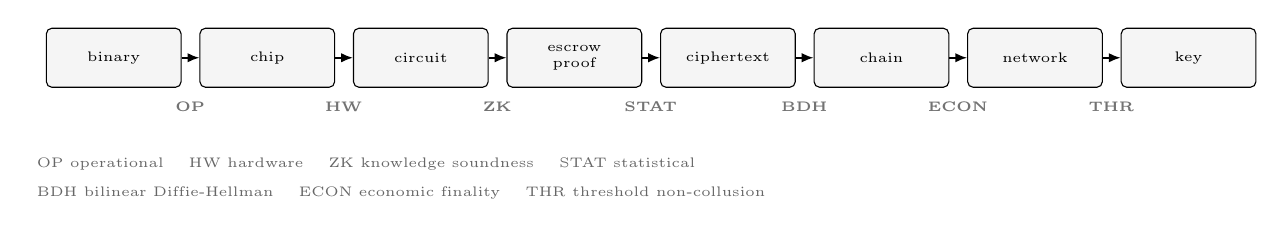
\begin{tikzpicture}[font=\tiny]
\foreach \i/\t in {0/{binary}, 1/{chip}, 2/{circuit}, 3/{escrow\\proof},
                   4/{ciphertext}, 5/{chain}, 6/{network}, 7/{key}} {
  \node[link, fill=black!4] (n\i) at (1.95*\i, 0) {\t};
}
\foreach \i in {0,...,6} {
  \pgfmathtruncatemacro\j{\i+1}
  \draw[msg] (n\i) -- (n\j);
}
\foreach \i/\m in {0/{OP}, 1/{HW}, 2/{ZK}, 3/{STAT}, 4/{BDH}, 5/{ECON},
                   6/{THR}} {
  \node[font=\tiny\bfseries, text=black!55] at (1.95*\i+0.97, -0.62) {\m};
}
\node[font=\tiny, text=black!60, anchor=west, align=left] at (-1.1, -1.35)
  {OP operational \quad HW hardware \quad ZK knowledge soundness \quad
   STAT statistical};
\node[font=\tiny, text=black!60, anchor=west, align=left] at (-1.1, -1.72)
  {BDH bilinear Diffie-Hellman \quad ECON economic finality \quad
   THR threshold non-collusion};
\end{tikzpicture}
\caption{The chain of custody. Each arrow carries the class of assumption that
protects it. Only three of the seven are cryptographic in the strict sense, and
the construction is only as strong as the weakest.}
\label{fig:trustchain}
\end{figure}

\begin{table}[h]
\centering
\small
\begin{tabular}{p{2.15cm}p{3.9cm}p{4.5cm}p{2.1cm}}
\toprule
Link & What it protects & Mechanism & Kind \\
\midrule
Binary to device &
  the code that runs is the code published &
  reproducible builds, store signature, attestation &
  operational \\
Chip to app &
  the passport is present, not copied &
  Equations \ref{eq:r2}, \ref{eq:r3}: chip signs a fresh bound challenge &
  hardware \\
App to circuit &
  the sealed bytes are the state-signed identity &
  Equations \ref{eq:r1}, \ref{eq:r6} share witness wires &
  cryptographic \\
Circuit to escrow &
  the committed secret is recoverable &
  Equations \ref{eq:feldman}, \ref{eq:recompute}, and $C_0 = hS$ &
  statistical \\
Escrow to storage &
  the platform cannot read what it holds &
  Equation \ref{eq:ibekey}, bilinear Diffie-Hellman &
  cryptographic \\
Request to chain &
  the request cannot be hidden or reordered &
  chain finality at depth &
  economic \\
Chain to network &
  no key exists without a public request &
  threshold derivation on an observed event &
  threshold \\
Key to disclosure &
  the opening becomes public &
  timelock beacon, threshold signature &
  threshold \\
Record to history &
  published history cannot be rewritten &
  Merkle inclusion plus anchoring &
  crypto, econ \\
\bottomrule
\end{tabular}
\caption{What secures each link. A reader tracing one enrollment passes through
all nine.}
\label{tab:trust}
\end{table}

\subsection{What is not cryptographic}
\label{sec:notcrypto}

Four assumptions carry weight and none of them is mathematics.

A1, threshold non-collusion, is what the construction rests on. It replaces the
custodial assumption of Section~\ref{sec:impossible}, and it is better only
because a user can inspect who operates the nodes and under which jurisdictions,
which they cannot do for a platform's internal key management.

A2, chain finality, is economic. It holds because reversing a settled block costs
more than an attacker gains, not because it is impossible.

A5, chip key non-extractability, is a hardware claim. Chips offering only passive
authentication are clonable from a data dump, which is why Equation~\ref{eq:r3}
is required rather than optional. Relay attacks remain possible even with it.

A6, client integrity, cannot be discharged by cryptography at all. The
application legitimately handles the plaintext. Section~\ref{sec:client} makes
violations detectable and never impossible.

\section{Design decisions}

Each of the following prevents a specific failure.

\begin{enumerate}
  \item \textbf{The shared secret is a uniform scalar, never the identity.} A
        Feldman commitment reveals $[s]P_1$, so committing to low-entropy data
        invites offline enumeration.
  \item \textbf{The verifier checks $C_0 = hS$ explicitly.} Making the commitment
        a circuit output stops the prover choosing it freely, and does not by
        itself bind it to the commitment the escrow proof uses.
  \item \textbf{Opened shares require Equation~\ref{eq:recompute}, not only
        Equation~\ref{eq:feldman}.} Checking a share against its commitment says
        nothing about the bytes stored beside it.
  \item \textbf{Recovery validates every candidate}, per
        Equation~\ref{eq:lagrange} and the check that follows it.
  \item \textbf{The challenge covers the complete statement before any opening},
        per Equation~\ref{eq:challenge}, so openings never influence selection.
  \item \textbf{A fresh polynomial per enrollment attempt.} Otherwise opened
        subsets from repeated attempts accumulate and cross the threshold.
  \item \textbf{The nullifier excludes the account identifier}, per
        Equation~\ref{eq:r4}. Including it would let one document enroll
        unlimited accounts.
  \item \textbf{Nobody validates the legal merit of a request.} No contract and
        no threshold network can read a court order. A fabricated justification
        is a credibility failure rather than a cryptographic one, detectable once
        the disclosure opens.
\end{enumerate}

One input remains unbound by construction. A liveness check comparing a selfie
against the chip photograph produces a single bit, and a circuit proving that bit
was set proves nothing about how it was produced. It is a client-trusted input
and must be labelled as one.

\section{The settlement layer}

The construction needs a chain for two jobs: anchoring the transparency record,
and carrying unseal requests where the escrow network can observe them. The
second constrains the first, because the request must land somewhere the network
already watches.

We take Gnosis Chain as the reference deployment. It is a proof-of-stake EVM
chain secured by more than 140{,}000 validators, a set second in size only to
Ethereum, reached by setting the stake per validator low enough for broad
participation. Blocks arrive about every five seconds, and the network tracks
Ethereum's upgrade path.

Two properties matter here beyond the usual ones.

\paragraph{Costs are flat in fiat.} Gas is paid in a stablecoin bridged one to
one, so an anchor costs the same next year as this year. A chain whose gas is
denominated in a volatile asset turns a ten-year anchoring commitment into an
unhedged position on that asset's price. For infrastructure meant to outlast
several market cycles, predictable beats cheap, and here it is both.

\paragraph{The escrow network already observes it.} Conditional key release
requires the network to evaluate a condition against chain state. Networks
capable of this watch specific chains, and a chain outside that set would need an
oracle to bridge it, reintroducing the trusted intermediary the design exists to
remove.

\paragraph{The honest trade.} Gnosis carries less economic weight behind finality
than Ethereum itself. For anchoring a transparency record, where the property
required is that published history cannot be quietly rewritten, that margin is
adequate. A deployment wanting stronger permanence can anchor continuously on the
settlement chain and push a periodic root to a higher-security chain through a
free timestamping aggregator, paying for the stronger guarantee only at the
slower cadence.

\section{Cost}

The commercial argument is that document verification happens on hardware the
user already owns. Constants: 50{,}000 gas for an anchor write, 120{,}000 for an
unseal request, gas at 2 gwei, 50 KB per enrollment record, storage at
\texttt{EUR} 0.021 per GB-month, and 0.3 seconds of processing per registration.
Deployments anchor on a size trigger or a time trigger, whichever fires first, so
the model takes the maximum of the two. Figure~\ref{fig:cost} and
Table~\ref{tab:costgrid} give the result.

\begin{figure}[t]
\centering
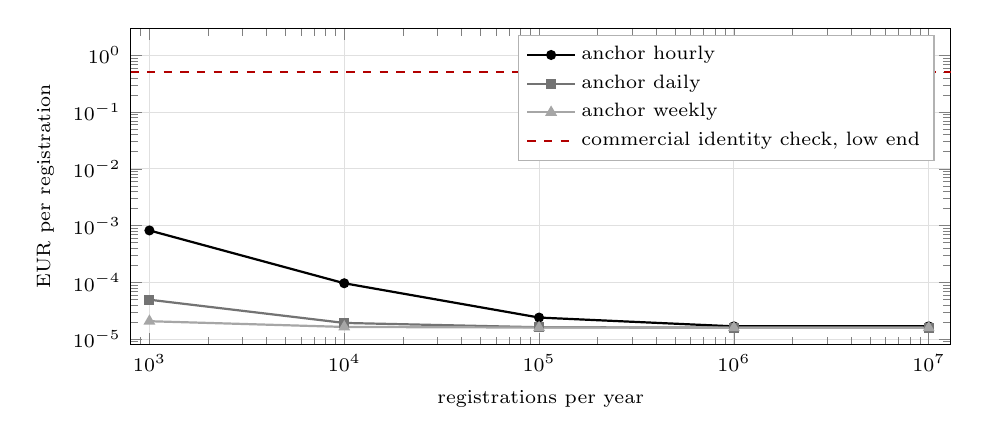
\begin{tikzpicture}
\begin{axis}[
  width=12cm, height=5.6cm,
  xmode=log, ymode=log,
  xlabel={registrations per year},
  ylabel={EUR per registration},
  xmin=800, xmax=1.3e7, ymin=8e-6, ymax=3,
  grid=major, grid style={black!12},
  tick label style={font=\scriptsize},
  label style={font=\scriptsize},
  legend style={font=\scriptsize, at={(0.98,0.98)}, anchor=north east,
                draw=black!30},
  legend cell align=left,
]
\addplot[black, line width=0.8pt, mark=*, mark size=1.4pt] coordinates {
  (1000,8.22e-4) (10000,9.65e-5) (100000,2.40e-5) (1000000,1.68e-5)
  (10000000,1.68e-5)
};
\addlegendentry{anchor hourly}
\addplot[black!55, line width=0.8pt, mark=square*, mark size=1.4pt] coordinates {
  (1000,4.95e-5) (10000,1.93e-5) (100000,1.62e-5) (1000000,1.60e-5)
  (10000000,1.60e-5)
};
\addlegendentry{anchor daily}
\addplot[black!35, line width=0.8pt, mark=triangle*, mark size=1.7pt] coordinates {
  (1000,2.07e-5) (10000,1.64e-5) (100000,1.60e-5) (1000000,1.59e-5)
  (10000000,1.59e-5)
};
\addlegendentry{anchor weekly}
\addplot[dashed, red!70!black, line width=0.7pt, mark=none] coordinates {
  (800,0.5) (1.3e7,0.5)
};
\addlegendentry{commercial identity check, low end}
\end{axis}
\end{tikzpicture}
\caption{Cost per registration against volume, log-log. Curves flatten once the
anchor cost amortises, after which storage dominates. The gap to commercial
identity verification is four to five orders of magnitude.}
\label{fig:cost}
\end{figure}

\begin{table}[h]
\centering
\begin{tabular}{lrrrrr}
\toprule
Anchor policy & 1k & 10k & 100k & 1M & 10M \\
\midrule
Hourly & $8.22 \times 10^{-4}$ & $9.65 \times 10^{-5}$ & $2.40 \times 10^{-5}$ & $1.68 \times 10^{-5}$ & $1.68 \times 10^{-5}$ \\
Daily  & $4.95 \times 10^{-5}$ & $1.93 \times 10^{-5}$ & $1.62 \times 10^{-5}$ & $1.60 \times 10^{-5}$ & $1.60 \times 10^{-5}$ \\
Weekly & $2.07 \times 10^{-5}$ & $1.64 \times 10^{-5}$ & $1.60 \times 10^{-5}$ & $1.59 \times 10^{-5}$ & $1.59 \times 10^{-5}$ \\
\bottomrule
\end{tabular}
\caption{EUR per registration by anchor cadence and annual volume.}
\label{tab:costgrid}
\end{table}

Total annual chain spend never exceeds \texttt{EUR} 9.20 across this grid, the
worst case being ten million registrations with hourly anchoring. Daily anchoring
at the same volume costs \texttt{EUR} 0.92 per year.

Chain cost is therefore not a design constraint at this scale, and anchor cadence
should be chosen for latency rather than price. Past roughly one hundred thousand
registrations a year, storage dominates, at which point the total for ten million
registrations is around \texttt{EUR} 160 annually.

The weakest constant is the 50 KB record size, derived from the structure of
pairing-based ciphertexts rather than measured. A four-fold error triples the
total and leaves the conclusion unchanged.

\section{The disclosure reference}

Property P3 asks that the published record carry a reference a human can check.
That reference is a free-form string, deliberately.

\paragraph{Why a string and not a structure.} The reference exists to be read by
a person holding a document and asking whether the two match. A rigid schema
would have to anticipate the request formats of every jurisdiction a platform
operates in, and would break the moment one changed. What the design fixes is not
the format but the binding: the hash of the string is committed on chain at
request time, so whatever it says, it was said before the outcome was known.

\paragraph{One convention worth requiring.} Requests reaching a platform fall
into two broad categories in most jurisdictions. Some are authorised by a judge
and carry a case identifier issued by a court registry, stable across the
proceeding. Others are issued directly by prosecutors or police under statutory
powers, carry only an internal administrative reference, and involve no judicial
authorisation at all. These differ enormously in the accountability they
represent.

A leading token naming the category is therefore worth requiring, even though
nothing parses it:

\begin{verbatim}
{ request: 'judicial <registry case identifier>' }
{ request: 'administrative <issuing body, internal reference>' }
\end{verbatim}

Published counts should separate the two. A single total that averages a judge's
order together with an administrative form tells a reader something untrue, and
the ratio between them is the number that actually describes a platform's
exposure.

\paragraph{What the reference does not prove.} A string is checkable only against
a registry the reader can query, and investigation records are frequently sealed.
Two facts partly compensate. The affected user acquires standing once their
account is suspended and can ask about their own case, which is the check by the
party most motivated to make it. And where an authority publishes aggregate
counts of orders issued, a platform's published total exceeding that figure is
proof of misstatement without needing any individual record.

\paragraph{The tension to resolve before deployment.} Statutory duties to comply
are sometimes paired with duties not to disclose. An architecture that publishes
by construction can collide with that, and the resolution determines whether the
on-chain commitment can be immediate or whether the whole request must sit behind
the timelock. That is a question for counsel in each jurisdiction, and it is the
first question a deployment should ask.

\section{Discussion}

\subsection{What CLAVE does not provide}
\label{sec:limits}

The implementation covers enrollment, the escrow proof, key derivation,
recovery, the unseal request and the timelocked disclosure. It does not cover
three parts. The credential circuit is evaluated in the clear, so no
zero-knowledge property holds and the binding of Equations~\ref{eq:r1}
to~\ref{eq:r6} is what the tests exercise. The settlement layer runs against a
mock that refuses to write to a real chain, because a deployment has to name a
contract first. The escrow network is a single process rather than a threshold
of independent nodes, which models the interface and not the custody.

Soundness figures are computed from Equation~\ref{eq:soundness} and are exact.
Cost figures come from the model of Section 8. Timings are host specific.

The escrow network can collude. A threshold of its nodes can derive keys without
a public request, and no observer would see anything. This is A1.

Networks capable of conditional key release are young. Asking one to hold
identity escrow for a decade is the principal deployment risk, larger in our
assessment than any cryptographic concern in this paper. Spreading shares across
several independent networks is the only lever that reduces it without recruiting
anyone, and it trades collusion resistance against the risk that one network
ceasing operation renders records permanently unopenable.

The credential circuit is the critical path and does not exist. Proving
Equations~\ref{eq:r1} through~\ref{eq:r6} together requires verifying a national
signature scheme and an authenticated encryption inside a circuit, which is
feasible and not cheap.

The client remains in the trusted base, because the application reads the
plaintext to seal it. Three measures make tampering detectable rather than
impossible. The app is open source. Android builds are reproducible, so anyone
can rebuild and compare the store binary byte for byte. Every release hash goes
to an append-only log, and the app refuses to run unless its own hash is in it,
so a build targeted at one user has to be published to work. Store attestation
proves the app to the platform's server, which stops a repackaged client from
enrolling. The iOS guarantee is weaker, because the store re-signs binaries and
byte comparison is impossible there, and a deployment must state that openly.

Passive chip authentication proves a country signed the data, never that the
physical chip is present. A passport data dump, from a breach or a hotel scan,
enrolls an account bound to that identity. The consequence is scoped: it
impersonates one person, so an unsealing names the wrong subject. It does not
break another user's seal and does not let the platform read anyone. Active or
Chip Authentication defeats the dump because a dump holds no private key. A
relay of a live chip defeats even that, and only a liveness check answers it.

Finally, CLAVE detects rather than prevents. A monitor that proves a platform
lied has produced a document. Whether that document carries a consequence is a
question of law.

\subsection{Related work}

Certificate Transparency~\cite{rfc9162} and CONIKS~\cite{coniks} establish
detection over prevention and supply the log machinery. Transparency
overlays~\cite{overlays} generalise it. Verifiable encryption of discrete
logarithms~\cite{camenisch} addressed escrow with sigma protocols two decades ago
and remains the closest prior treatment of the enrollment problem.
Identity-based encryption~\cite{bf} supplies Equation~\ref{eq:ibekey}. Threshold
timelock encryption~\cite{tlock} supplies the disclosure mechanism. Shamir
sharing~\cite{shamir} and Feldman commitments~\cite{feldman} supply the escrow
proof, and Fiat-Shamir~\cite{fiatshamir} makes it non-interactive.

\subsection{Conclusion}

A platform that holds your identity cannot prove it did not read it. That is not
an engineering shortfall and no amount of logging repairs it.

CLAVE follows from taking that seriously. Seal on the user's device. Hold no
master key. Make every release depend on a public act the platform cannot perform
privately. What remains is an availability question, and availability is
something anyone can observe.

The cryptography is the straightforward part. Deciding what not to hold is the
rest of it.

\section*{Author contributions}

R.S. designed the construction and set the evidence standard. Design review and
drafting used large language model assistance under human direction, with
independent models used to review each other's conclusions. The author is
responsible for all content.

\section*{Availability}

The reference implementation, the cost model, and the reproduction harness are
at \url{https://clave.sospedra.me} and in the repository at
\url{https://github.com/sospedra/sospedra.me}. Running
\texttt{scripts/reproduce.mts} emits Table~\ref{tab:soundness},
Figure~\ref{fig:cheating} and Table~\ref{tab:measured}. Running
\texttt{scripts/cost-model.mts} emits Table~\ref{tab:costgrid} and
Figure~\ref{fig:cost}. Running \texttt{pnpm test} exercises the protocol
end to end against a mock chain and a mock beacon.

\begin{thebibliography}{10}

\bibitem{doormats}
H. Abelson \emph{et al.}, ``Keys under doormats: mandating insecurity by
requiring government access to all data and communications,''
\emph{Journal of Cybersecurity}, vol. 1, no. 1, pp. 69--79, 2015.

\bibitem{rfc9162}
B. Laurie, E. Messeri, and R. Stradling, ``Certificate Transparency version
2.0,'' RFC 9162, Dec. 2021.

\bibitem{coniks}
M. S. Melara, A. Blankstein, J. Bonneau, E. W. Felten, and M. J. Freedman,
``CONIKS: bringing key transparency to end users,'' in \emph{Proc. USENIX
Security}, 2015, pp. 383--398.

\bibitem{overlays}
M. Chase and S. Meiklejohn, ``Transparency overlays and applications,'' in
\emph{Proc. ACM CCS}, 2016, pp. 168--179.

\bibitem{bf}
D. Boneh and M. Franklin, ``Identity-based encryption from the Weil pairing,''
in \emph{Proc. CRYPTO}, 2001, pp. 213--229.

\bibitem{shamir}
A. Shamir, ``How to share a secret,'' \emph{Communications of the ACM},
vol. 22, no. 11, pp. 612--613, 1979.

\bibitem{feldman}
P. Feldman, ``A practical scheme for non-interactive verifiable secret
sharing,'' in \emph{Proc. IEEE FOCS}, 1987, pp. 427--438.

\bibitem{fiatshamir}
A. Fiat and A. Shamir, ``How to prove yourself: practical solutions to
identification and signature problems,'' in \emph{Proc. CRYPTO}, 1986,
pp. 186--194.

\bibitem{camenisch}
J. Camenisch and V. Shoup, ``Practical verifiable encryption and decryption of
discrete logarithms,'' in \emph{Proc. CRYPTO}, 2003, pp. 126--144.

\bibitem{tlock}
N. Gailly, K. Melissaris, and Y. Romailler, ``tlock: practical timelock
encryption from threshold BLS,'' IACR ePrint 2023/189, 2023.

\end{thebibliography}

\end{document}
